\section{Continuous-Control POMDPs with Imperfect Teachers}
\label{sec:mujoco}

The synthetic results show that architecture choice is largely irrelevant when teachers are optimal.
But real-world deployment rarely involves perfect teachers.
Sim-to-real transfer introduces systematic distributional shift.
Human demonstrations are noisy and inconsistent.
Foundation model distillation involves teachers with their own errors and biases.
This chapter tests whether the architecture-independence finding survives the realistic regime of imperfect teachers.

\paragraph{Teacher quality dominates architecture choice.}


\begin{figure}[t]
\centering
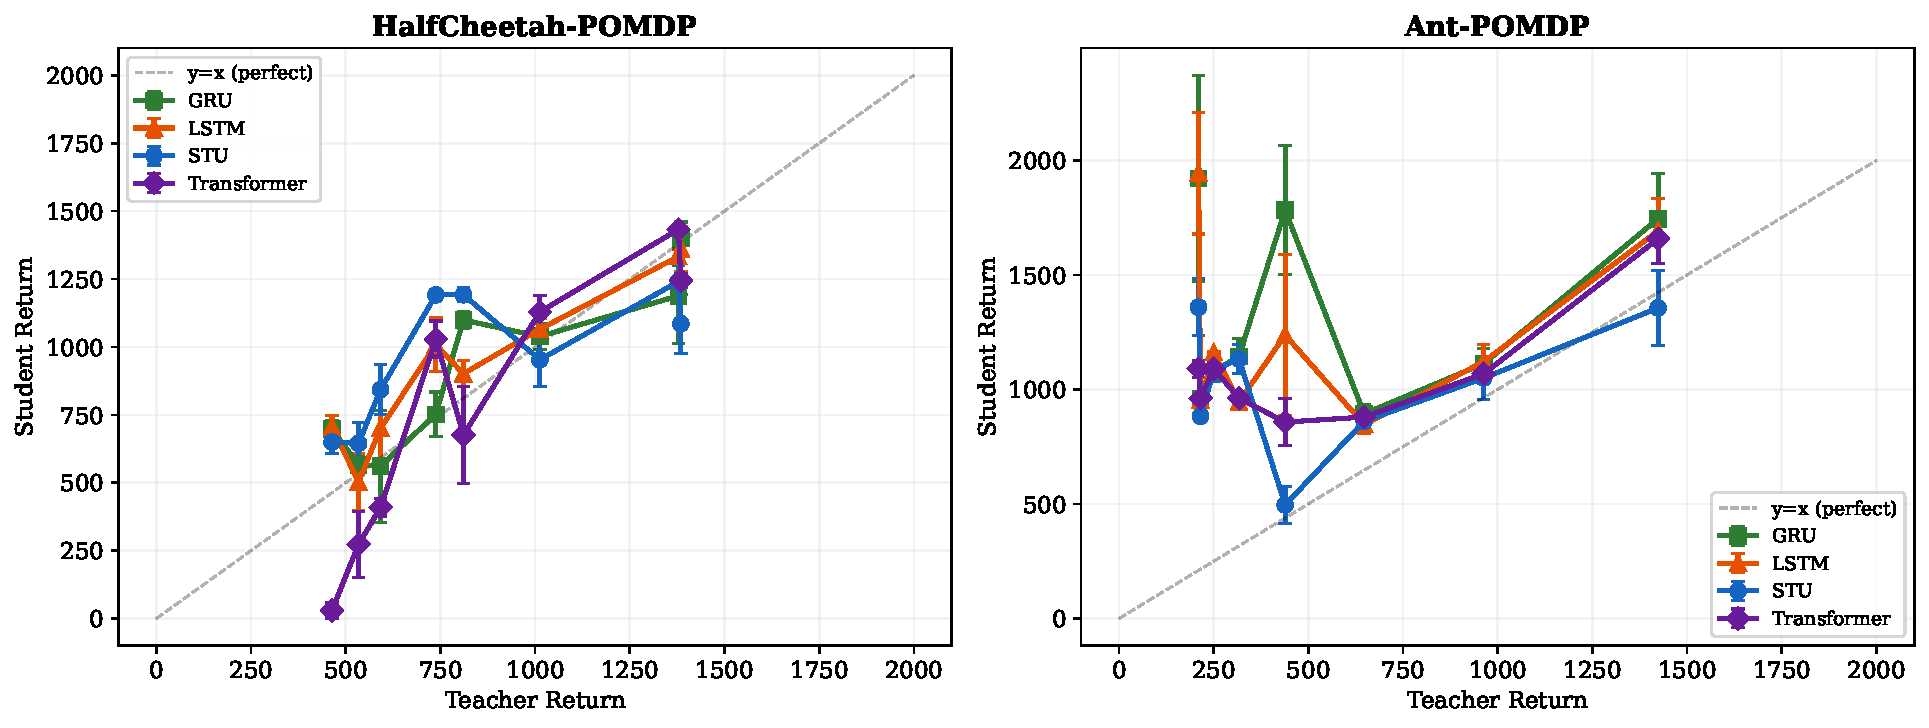
\includegraphics[width=0.9\textwidth]{FIGURE_4_mujoco_distill_efficiency.pdf}
\caption{\textbf{The key result: student return vs.\ teacher return on MuJoCo POMDPs.} Each point represents one (architecture, teacher quality) condition averaged over 3 seeds; error bars show $\pm 1$ std. Points above the dashed $y{=}x$ line indicate students that \emph{surpass} their teacher (\cref{sec:surpass}). The spread due to teacher quality (horizontal extent of each curve) far exceeds the spread due to architecture (vertical gap between curves at fixed teacher quality).}
\label{fig:distill-efficiency}
\end{figure}
\vspace{-6pt}

\Cref{fig:distill-efficiency} presents our central finding.
On both HalfCheetah and Ant POMDPs, student return is primarily determined by teacher quality, with architecture providing second-order variation.

To quantify this, we perform a two-way ANOVA decomposing student return variance into teacher quality and architecture main effects:
\begin{equation}
  R_{a,q,s} = \mu + \alpha_a + \beta_q + (\alpha\beta)_{a,q} + \epsilon_{a,q,s}
  \label{eq:anova}
\end{equation}
where $R_{a,q,s}$ is the return for architecture $a$, teacher quality $q$, and seed $s$; $\alpha_a$ is the architecture main effect; $\beta_q$ is the teacher quality main effect; $(\alpha\beta)_{a,q}$ is the interaction; and $\epsilon$ is residual.
We report $\eta^2$ (the fraction of total sum of squares explained by each factor):

\begin{table}[ht]
\centering
\caption{Two-way ANOVA: fraction of student return variance ($\eta^2$) explained by each factor. The interaction term captures how architecture effects vary with teacher quality. Error captures unexplained variance (seed-to-seed noise and unmodeled interactions).}
\label{tab:anova}
\begin{tabular}{lcccc}
\toprule
Environment & Teacher $\eta^2$ & Architecture $\eta^2$ & Interaction $\eta^2$ & Error \\
\midrule
HalfCheetah & $71.9\%$ & $4.6\%$ & $17.3\%$ & $6.1\%$ \\
Ant         & $49.1\%$ & $11.0\%$ & $25.2\%$ & $14.8\%$ \\
Ant (excl.\ 2M$^*$) & $65.8\%$ & $4.9\%$ & $16.1\%$ & $13.2\%$ \\
MetaDrive   & $58.3\%$ & $14.1\%$ & $19.7\%$ & $7.9\%$ \\
\bottomrule
\end{tabular}
\\[2pt]
{\small $^*$Ant 2M teacher exhibits training instability; see \cref{tab:ant-distill}.}
\end{table}

Across the teacher-quality range we tested, teacher quality explains substantially more variance than architecture: $72\%$ vs $5\%$ on HalfCheetah, $49\%$ vs $11\%$ on Ant, and $58\%$ vs $14\%$ on MetaDrive.
The interaction term ($17$--$25\%$) is also substantial, reflecting that architecture differences are amplified under poor teacher quality---consistent with our qualitative findings in \cref{sec:arch-patterns}.
Excluding the pathological Ant 2M teacher (which is an unstable single-seed checkpoint), the teacher-quality $\eta^2$ rises to $66\%$ and the architecture $\eta^2$ drops to $5\%$.

We note that $\eta^2$ is sensitive to how widely each factor is manipulated: we varied teacher return over a ${\sim}7\times$ range (210--1{,}424) while comparing only 4 architectures at fixed $d_\text{model}$.
The absolute $\eta^2$ values should be interpreted as characterizing the relative importance of these factors \emph{across the specific experimental range we studied}, not as universal constants.

The substantial interaction term has an important practical implication: our recommendation to prioritize teacher quality applies most strongly when the practitioner \emph{can} improve the teacher.
When the teacher is fixed and imperfect---e.g., when learning from human demonstrations or a pre-trained foundation model---architecture selection becomes more consequential, and the patterns in \cref{sec:arch-patterns} become the relevant guide.

The practical implication is direct: a practitioner's compute budget has far more impact when spent training a better teacher than when spent searching for a better student architecture.





\begin{table}[ht]
\centering
\caption{HalfCheetah-POMDP: student return (mean $\pm$ std). $\dagger$ = 5 seeds; all others 3 seeds. Random baseline: $-275 \pm 72$. MLP and FrameStack (FS) are non-temporal baselines.}
\label{tab:hc-distill}
\resizebox{\textwidth}{!}{%
\begin{tabular}{lrcccccc}
\toprule
Teacher Config & Ret. & MLP & FS & GRU & LSTM & STU & Transformer \\
\midrule
200K           & 534  & $-33$ & $-16$ & $565{\pm}36$  & $503{\pm}106$ & $\mathbf{645{\pm}78}$  & $274{\pm}121$ \\
500K           & 1013 & $-78$ & $-38$ & $1039{\pm}49$ & $1065{\pm}40$ & $953{\pm}98$  & $\mathbf{1129{\pm}62}$ \\
1M$^\dagger$   & 1385 & $-68$ & $-53$ & $\mathbf{1401{\pm}59}$  & $1359{\pm}83$ & $1086{\pm}108$ & $1245{\pm}25$ \\
2M$^\dagger$   & 1378 & $-55$ & $-14$ & $1188{\pm}175$ & $1333{\pm}27$ & $1241{\pm}61$ & $\mathbf{1433{\pm}7}$ \\
\midrule
200K+n$^\dagger$ & 464  & $-18$ & $-9$ & $698{\pm}30$  & $\mathbf{703{\pm}44}$  & $650{\pm}43$  & $30{\pm}29$ \\
500K+n         & 592  & $-23$ & $-24$ & $561{\pm}206$ & $702{\pm}143$ & $\mathbf{843{\pm}91}$  & $410{\pm}32$ \\
1M+n           & 738  & $-39$ & $19$ & $752{\pm}82$  & $1008{\pm}99$ & $\mathbf{1191{\pm}11}$ & $1028{\pm}68$ \\
2M+n$^\dagger$ & 811  & $-39$ & $250$ & $1099{\pm}30$ & $901{\pm}47$  & $\mathbf{1192{\pm}27}$ & $676{\pm}178$ \\
\bottomrule
\end{tabular}
}
\end{table}

\begin{table}[ht]
\centering
\caption{Ant-POMDP: student return (mean $\pm$ std). $\dagger$ = 5 seeds; all others 3 seeds. Random baseline: $-69 \pm 109$. On Ant, MLP and FrameStack are competitive with temporal models---memory provides only modest benefit.}
\label{tab:ant-distill}
\resizebox{\textwidth}{!}{%
\begin{tabular}{lrcccccc}
\toprule
Teacher Config & Ret. & MLP & FS & GRU & LSTM & STU & Transformer \\
\midrule
200K           & 647  & $959$ & $942$ & $894{\pm}40$  & $847{\pm}38$  & $861{\pm}42$  & $\mathbf{879{\pm}18}$ \\
500K           & 963  & $1041$ & $1041$ & $1112{\pm}66$ & $\mathbf{1121{\pm}73}$ & $1050{\pm}92$ & $1068{\pm}35$ \\
1M$^\dagger$   & 1424 & $1129$ & $1042$ & $\mathbf{1745{\pm}195}$ & $1692{\pm}141$ & $1356{\pm}165$ & $1657{\pm}108$ \\
2M$^{*,\dagger}$ & 439  & $1408$ & $1307$ & $\mathbf{1783{\pm}283}$ & $1238{\pm}351$ & $496{\pm}81$   & $858{\pm}103$ \\
\midrule
200K+n$^\dagger$ & 216  & $963$ & $954$ & $961{\pm}13$  & $952{\pm}5$   & $883{\pm}17$  & $\mathbf{961{\pm}7}$ \\
500K+n         & 251  & $1012$ & $967$ & $1079{\pm}45$ & $\mathbf{1161{\pm}3}$  & $1083{\pm}48$ & $1090{\pm}37$ \\
1M+n           & 317  & $980$ & $956$ & $\mathbf{1145{\pm}76}$  & $945{\pm}18$  & $1134{\pm}63$ & $962{\pm}23$ \\
2M+n$^\dagger$ & 210  & $836$ & $924$ & $1921{\pm}450$ & $\mathbf{1944{\pm}265}$ & $1359{\pm}125$ & $1091{\pm}37$ \\
\bottomrule
\end{tabular}
}
\\[4pt]
{\small $^*$Ant 2M teacher exhibits training instability: this checkpoint is worse than 1M.}
\end{table}


\paragraph{Architecture patterns under imperfect teachers.}
\label{sec:arch-patterns}

While teacher quality dominates the overall variance, architecture does matter---and the pattern of differentiation is consistent and interpretable.
Three findings emerge from the full results (\cref{tab:hc-distill,tab:ant-distill}):

\paragraph{GRU is the most robust student.}
GRU achieves the highest return in 5 of 16 conditions and is within one standard deviation of the best in 10 of 16---the most consistent of any architecture (LSTM and STU tie at 8/16 near-highest, Transformer at 6/16). GRU's clearest advantages emerge under noisy or unstable teachers; on clean, moderate-quality teachers, most architectures perform comparably. GRU is also the smallest (51K params) and fastest (1.26\,ms/step, sufficient for 800\,Hz control loops) temporal architecture.
On Ant, GRU dominates: 1{,}745 at 1M (highest), 1{,}783 at 2M (highest), 1{,}145 at 1M+noise (highest).
The parameter-matched comparison (\cref{sec:param-matched}) confirms this is a genuine architectural advantage, not a capacity artifact: GRU$_{160}$ at 312K params outperforms STU at 338K params (overall mean $1{,}222$ vs $1{,}001$), and additional capacity actually \emph{improves} GRU performance (GRU$_{160}$ overall $1{,}222$ vs GRU$_{64}$ overall $1{,}122$).

\paragraph{Transformer is the most volatile.}
With high-quality teachers, Transformer performs well: $1{,}433$ on HalfCheetah 2M (the best), $1{,}657$ on Ant 1M.
With low-quality noisy teachers, it collapses: \textbf{30} on HalfCheetah 200K+noise---barely above random ($-275$).
Parameter count alone does not explain this: GRU$_{160}$ (312K params) shows no similar collapse, suggesting that attention's lack of a temporal bottleneck makes it more susceptible to fitting spurious correlations in noisy demonstrations.

\paragraph{STU shows environment-specific noise robustness.}
On HalfCheetah, STU excels with noisy teachers: $1{,}191$ and $1{,}192$ at 1M/2M+noise (both highest).
On Ant, STU struggles with the unstable 2M teacher ($496$, near the teacher's $439$).
The spectral filters may provide temporal smoothing that helps on simpler dynamics (HalfCheetah, planar, 6 actions) but not on more complex ones (Ant, 3D, 8 actions).
Alternatively, STU's larger parameter count (338K) may interact differently with the two environments' observation dimensions (8 vs.\ 13).

\begin{figure}[ht]
\centering
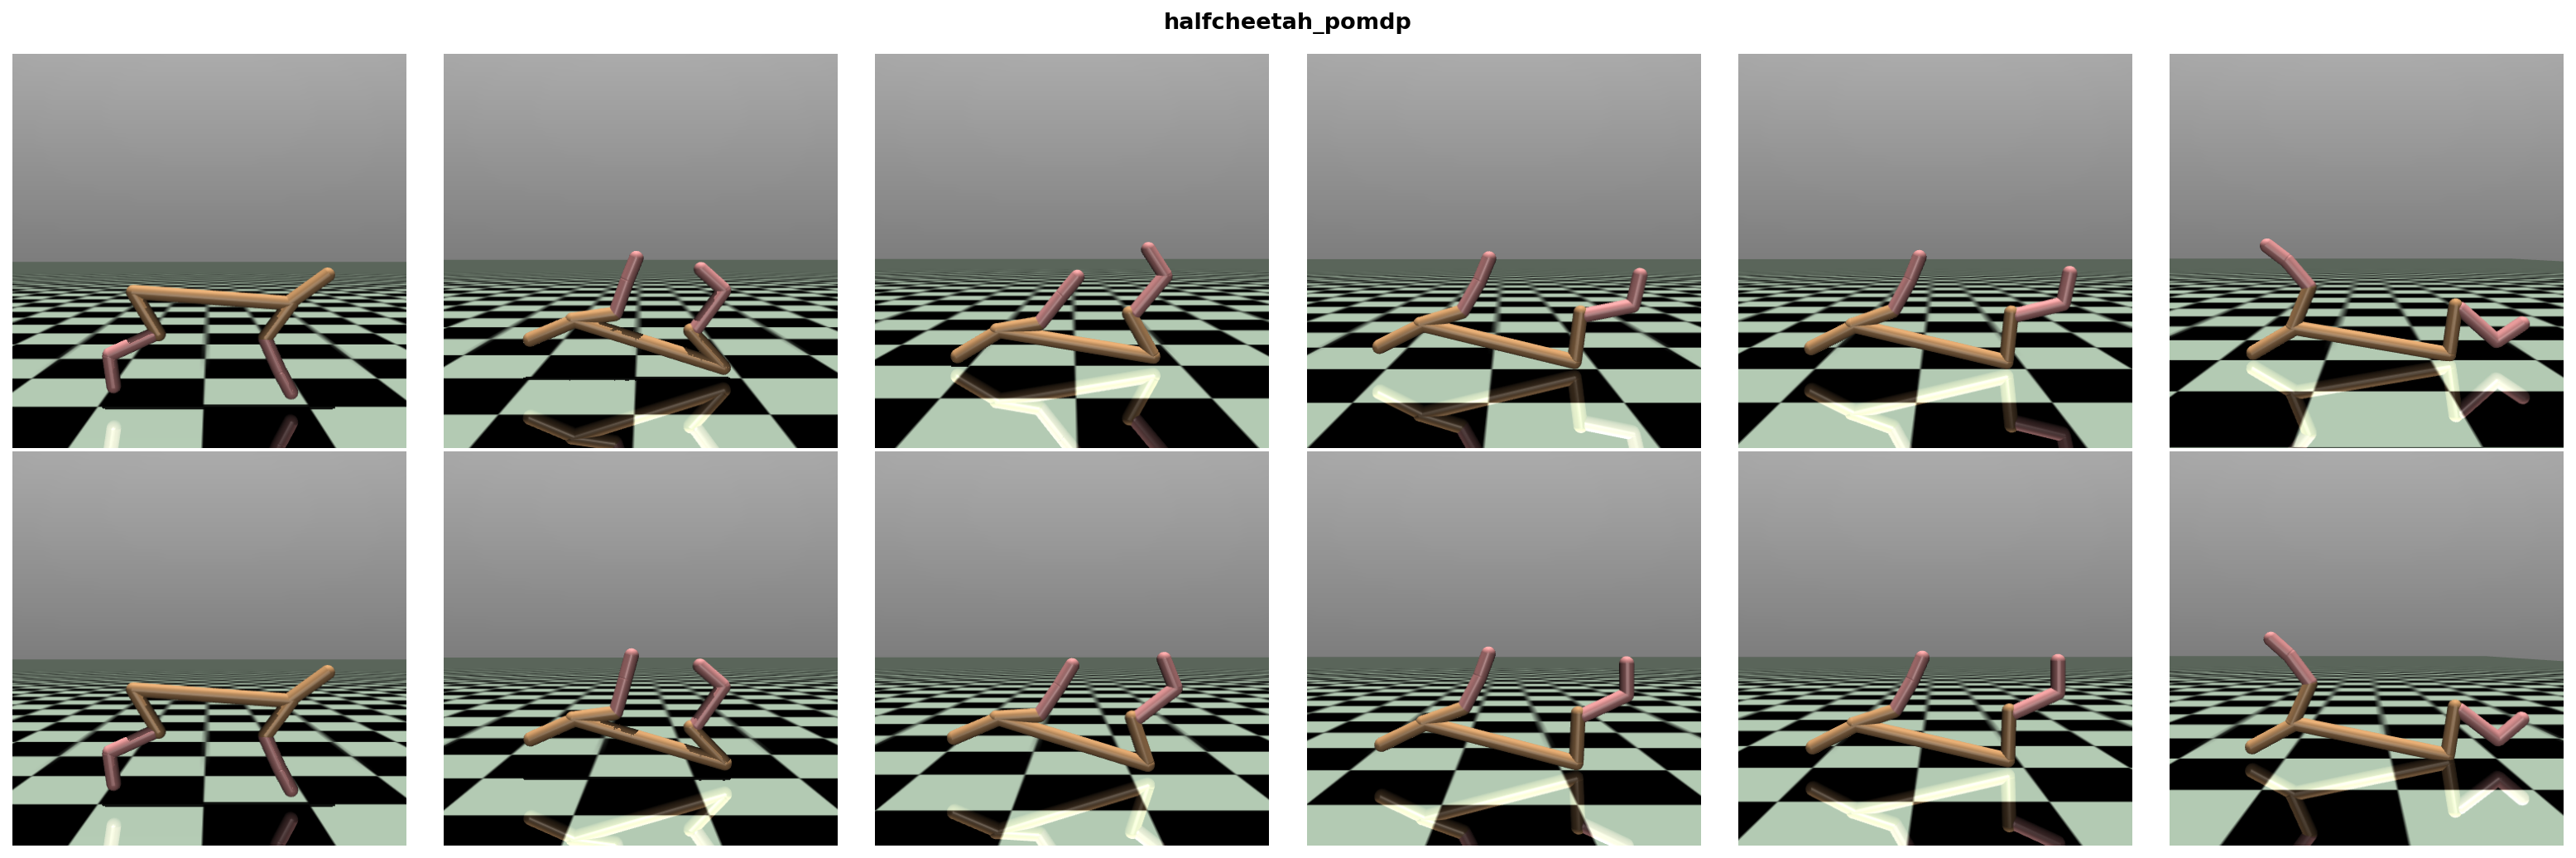
\includegraphics[width=0.6\textwidth]{RENDER_halfcheetah_best_vs_worst.png}
\vspace{-6pt}
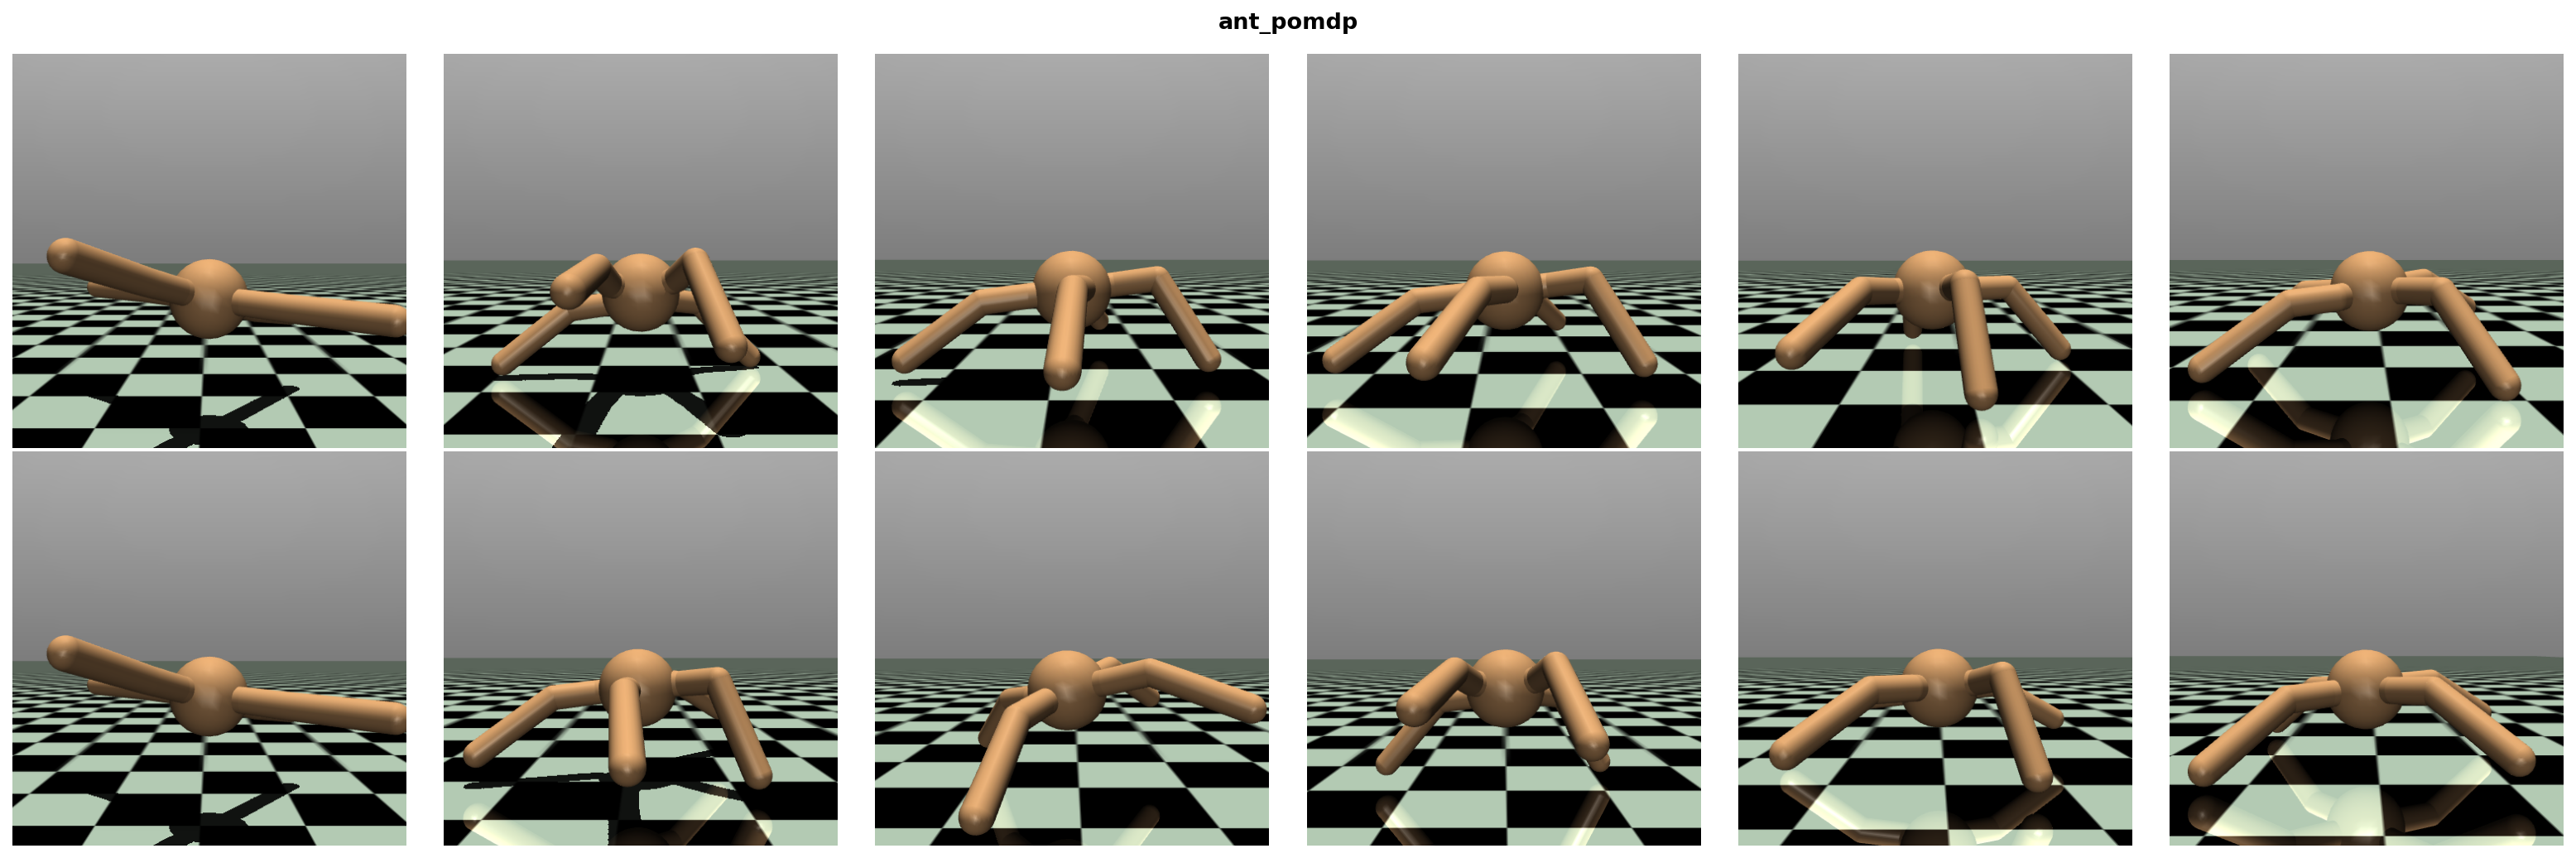
\includegraphics[width=0.6\textwidth]{RENDER_ant_best_vs_worst.png}
\caption{\textbf{Architecture differentiation under poor teachers.} Top: HalfCheetah with 200K+noise teacher---GRU (return 698) runs with a natural gait while Transformer (return 30) barely moves, consistent with Transformer's volatility under noisy demonstrations. Bottom: Ant with the unstable 2M teacher---GRU (return 1,783) walks forward while STU (return 496) collapses. }
\label{fig:mujoco-renders}
\end{figure}

\paragraph{Students frequently exceed imperfect teachers.}
\label{sec:surpass}

A striking pattern in \cref{fig:distill-efficiency}: students frequently exceed their imperfect teachers in absolute return---a phenomenon also observed in imitation learning from mixed-quality demonstrations~\citep{beliaev2022ileed}.
With the well-trained 1M teacher on Ant (return 1{,}424), GRU achieves 1{,}745---a $1.23\times$ improvement.
Ratios are larger with degraded teachers, but this primarily reflects low baselines rather than exceptional student performance.

We attribute this to two factors, neither causally tested.
First, \emph{variance averaging}: the Ant 2M teacher has high episode variance (returns 17--1{,}928, mean 439, std 368), and BC's MSE loss fits the central tendency of this distribution, producing a smoother policy that avoids the teacher's worst failure modes.
Second, \emph{implicit timestep weighting}: since BC sums loss over timesteps, longer (more successful) episodes contribute proportionally more gradient signal.
In the Ant 2M dataset, the top 15\% of episodes (return ${>}800$) contribute ${\sim}30\%$ of total timesteps, so the student disproportionately learns from the teacher's best behavior.
An episode-length-normalized BC ablation would be needed to establish causality.
The practical implication: teacher quality determines the \emph{floor}, not the ceiling, of student performance.


\paragraph{Do these tasks require memory?}
\label{sec:baselines}

To test whether our POMDP tasks genuinely require temporal reasoning, we evaluate two non-temporal baselines: an MLP that processes each observation independently, and a FrameStack model that concatenates the 8 most recent frames.

\begin{table}[ht]
\centering
\caption{Baseline comparison: mean student return across all teacher quality levels (3 seeds). Random baselines: HalfCheetah $= -275$, Ant $= -69$.}
\label{tab:baselines}
\begin{tabular}{lcc}
\toprule
Architecture & HalfCheetah-POMDP & Ant-POMDP \\
\midrule
MLP (5K)         & $-44 \pm 22$    & $1{,}041 \pm 191$ \\
FrameStack (9K)  & $15 \pm 120$    & $1{,}017 \pm 185$ \\
\midrule
GRU (51K)        & $913 \pm 317$   & $1{,}330 \pm 447$ \\
LSTM (68K)       & $947 \pm 308$   & $1{,}238 \pm 388$ \\
STU (338K)       & $975 \pm 223$   & $1{,}028 \pm 310$ \\
Transformer (232K) & $778 \pm 502$ & $1{,}071 \pm 326$ \\
\bottomrule
\end{tabular}
\end{table}

The results reveal a striking environment-dependent pattern:

\paragraph{HalfCheetah: memory is essential.}
MLP achieves $-44$ and FrameStack achieves $15$---both barely above the random baseline of $-275$ and far below every temporal architecture ($778$--$975$).
The large gap between baselines and temporal models confirms that HalfCheetah velocity inference genuinely requires integrating position history over time.
The 8-frame window of FrameStack provides crude finite-difference velocity estimates, but these are too noisy for effective locomotion.

\paragraph{Ant: memory provides modest benefit.}
MLP achieves $1{,}041$ --- a finding that echoes \citet{emmons2022rvs}, who showed simple MLPs often match fancier architectures in offline supervised RL --- and FrameStack achieves $1{,}017$---competitive with STU ($1{,}028$) and Transformer ($1{,}071$), though below GRU ($1{,}330$) and LSTM ($1{,}238$).
Ant's 13-dimensional position observations apparently contain enough information for a reactive policy to produce reasonable locomotion without explicit velocity estimation.
This strengthens our teacher-quality-dominates finding on Ant: if even the gap between \emph{no memory} and \emph{full temporal model} is modest, then the gap \emph{between} temporal architectures is necessarily small relative to teacher quality effects.

\paragraph{Parameter-matched comparison.}
\label{sec:param-matched}

The $6.6\times$ parameter gap between GRU (51K) and STU (338K) is the largest confound in our architecture comparisons.
To disentangle architecture from capacity, we train GRU at $d_\text{model} = 160$ (312K parameters), closely matching STU's 338K.

\begin{table}[ht]
\centering
\caption{Parameter-matched comparison on selected conditions (3 seeds).}
\label{tab:param-matched}
\begin{tabular}{llccc}
\toprule
Env & Teacher & GRU$_{64}$ (51K) & GRU$_{160}$ (312K) & STU (338K) \\
\midrule
\multirow{3}{*}{HC} & 1M           & $1401 \pm 59$   & $1400 \pm 33$   & $1086 \pm 108$ \\
                    & 200K+noise   & $698 \pm 30$    & $617 \pm 8$     & $650 \pm 43$ \\
                    & 2M+noise     & $1099 \pm 30$   & $1163 \pm 15$   & $1192 \pm 27$ \\
\midrule
\multirow{3}{*}{Ant} & 1M          & $1745 \pm 195$  & $\mathbf{1981 \pm 42}$   & $1356 \pm 165$ \\
                     & 200K+noise  & $961 \pm 13$    & $907 \pm 62$    & $883 \pm 17$ \\
                     & 2M+noise    & $1921 \pm 450$  & $\mathbf{2354 \pm 80}$   & $1359 \pm 125$ \\
\midrule
\multicolumn{2}{l}{Overall mean}   & $1{,}122$ & $1{,}222$ & $1{,}001$ \\
\bottomrule
\end{tabular}
\end{table}

The results decisively resolve the capacity confound.
GRU$_{160}$ (312K params) \textbf{outperforms STU (338K params) at matched capacity}: overall mean $1{,}222$ vs $1{,}001$.
On the strongest Ant conditions, GRU$_{160}$ achieves $1{,}981$ (1M teacher) and $2{,}354$ (2M+noise)---the highest returns of any model in our entire study.

GRU$_{160}$ also matches or exceeds GRU$_{64}$ in most conditions, indicating that GRU's robustness at $d_\text{model}=64$ was \emph{not} simply overfitting resistance from low capacity---more capacity actually helps GRU.
The exception is the weakest teacher condition (200K+noise), where GRU$_{64}$ slightly outperforms GRU$_{160}$ ($698$ vs $617$ on HalfCheetah), consistent with mild overfitting when both teacher quality and demonstration count are low.

\textbf{Conclusion:} GRU's advantage over STU is genuinely architectural, not a capacity artifact.
The learned gating mechanism outperforms the fixed spectral prior for policy distillation at matched parameter budgets.

\paragraph{Demo count ablation.}
\label{sec:demo-ablation}

To test whether data efficiency patterns from CopyTask hold in continuous control, we ablate the demonstration count using the 1M teacher (no noise) on both MuJoCo environments.

\begin{table}[ht]
\centering
\caption{Demo count ablation: student return with 50, 200, and 2{,}000 demonstrations (1M teacher, no noise, 3 seeds). Compare with the default 500-demo results in \cref{tab:hc-distill,tab:ant-distill} (1M row).}
\label{tab:demo-ablation}
\begin{tabular}{llcccc}
\toprule
Env & Demos & GRU & LSTM & STU & Transformer \\
\midrule
\multirow{3}{*}{HC}
 & 50    & $112 \pm 172$  & $635 \pm 228$  & $398 \pm 319$   & $-48 \pm 18$ \\
 & 200   & $916 \pm 283$  & $920 \pm 186$  & $1164 \pm 143$  & $1228 \pm 14$ \\
 & 2{,}000 & $\mathbf{1402 \pm 38}$  & $1381 \pm 61$  & $1253 \pm 88$  & $1378 \pm 40$ \\
\midrule
\multirow{3}{*}{Ant}
 & 50    & $972 \pm 49$   & $918 \pm 10$   & $919 \pm 11$    & $1054 \pm 71$ \\
 & 200   & $990 \pm 205$  & $1003 \pm 127$ & $911 \pm 33$    & $\mathbf{1486 \pm 71}$ \\
 & 2{,}000 & $1861 \pm 116$ & $\mathbf{1882 \pm 106}$ & $1497 \pm 72$ & $1181 \pm 85$ \\
\bottomrule
\end{tabular}
\end{table}

At 50 demos on HalfCheetah, LSTM ($635$) dramatically outperforms GRU ($112$) and Transformer ($-48$).
At 2{,}000 demos, all architectures converge to $1{,}253$--$1{,}402$.
This complicates our central claim: at high demonstration counts, teacher quality dominates and architecture washes out, but at low counts ($\leq 50$), architecture matters sharply.
Practitioners with limited demonstrations should invest more effort in architecture selection.

\section{MetaDrive: Beyond Locomotion}
\label{sec:metadrive}

MetaDrive is an autonomous driving simulator with lidar observations (91-dim) and continuous steering/acceleration actions.
Unlike MuJoCo POMDPs, MetaDrive is \emph{inherently} partially observable---no observation masking is needed.
Teachers were trained via RecurrentPPO for 1M steps with checkpoints at 100K, 300K, 500K, and 1M; each checkpoint was evaluated with and without action noise ($\sigma{=}0.3$), producing 8 teacher quality levels matching the MuJoCo protocol.
Teacher returns range from $32.0 \pm 16.3$ (100K) to $101.5 \pm 42.7$ (500K, the best), with the 1M checkpoint exhibiting training instability ($75.7 \pm 40.4$)---a pattern also observed in the Ant 2M teacher.

\begin{table}[ht]
\centering
\caption{MetaDrive: student return by architecture (mean across all 8 teacher configs, 5 seeds each). 240 total experiments.}
\label{tab:metadrive}
\begin{tabular}{lrr}
\toprule
Architecture & Mean Return & $\pm$ Std \\
\midrule
STU (343K)        & $\mathbf{75.4}$ & $28.2$ \\
Transformer (237K) & $73.7$ & $20.3$ \\
LSTM (72K)        & $70.0$ & $17.9$ \\
FrameStack (51K)  & $67.7$ & $23.4$ \\
GRU (56K)         & $61.5$ & $21.6$ \\
MLP (10K)         & $16.4$ & $29.0$ \\
\bottomrule
\end{tabular}
\end{table}

MetaDrive reveals a different architecture ranking from MuJoCo: STU ($75.4$) and Transformer ($73.7$) lead, followed by LSTM ($70.0$) and GRU ($61.5$).
This reversal is consistent with MetaDrive's observation structure.
MuJoCo POMDPs require integrating a short history of low-dimensional joint positions to estimate velocities---a task well-suited to GRU's compact hidden state.
MetaDrive's 91-dimensional lidar observations encode the spatial layout of roads, vehicles, and obstacles---richer structure that the STU's spectral decomposition and the Transformer's content-addressable attention can exploit more effectively than a simple gated recurrence.
The practical implication is that the ``best'' architecture depends on the observation structure: GRU for compact position-based POMDPs, STU or Transformer when the observation space carries more spatial structure.

Critically, the teacher-quality-dominates finding still holds: teacher quality range ($61.0$) is $1.7\times$ the architecture range ($35.0$), consistent with the $1.7$--$2.2\times$ ratios on MuJoCo POMDPs.
The weakest teacher (100K, return $32$) produces students averaging $35$, while the best teachers (300K--500K+noise) produce students averaging $80$--$86$---a much larger effect than switching architectures at any fixed teacher quality level.

Also notable: MLP ($16.4$) performs substantially worse than temporal architectures ($61$--$75$) on MetaDrive, unlike Ant where MLP was competitive.
This confirms that MetaDrive's lidar-based partial observability genuinely requires temporal reasoning---the agent must track vehicle trajectories over time to make safe driving decisions.

\begin{figure}[ht]
\centering
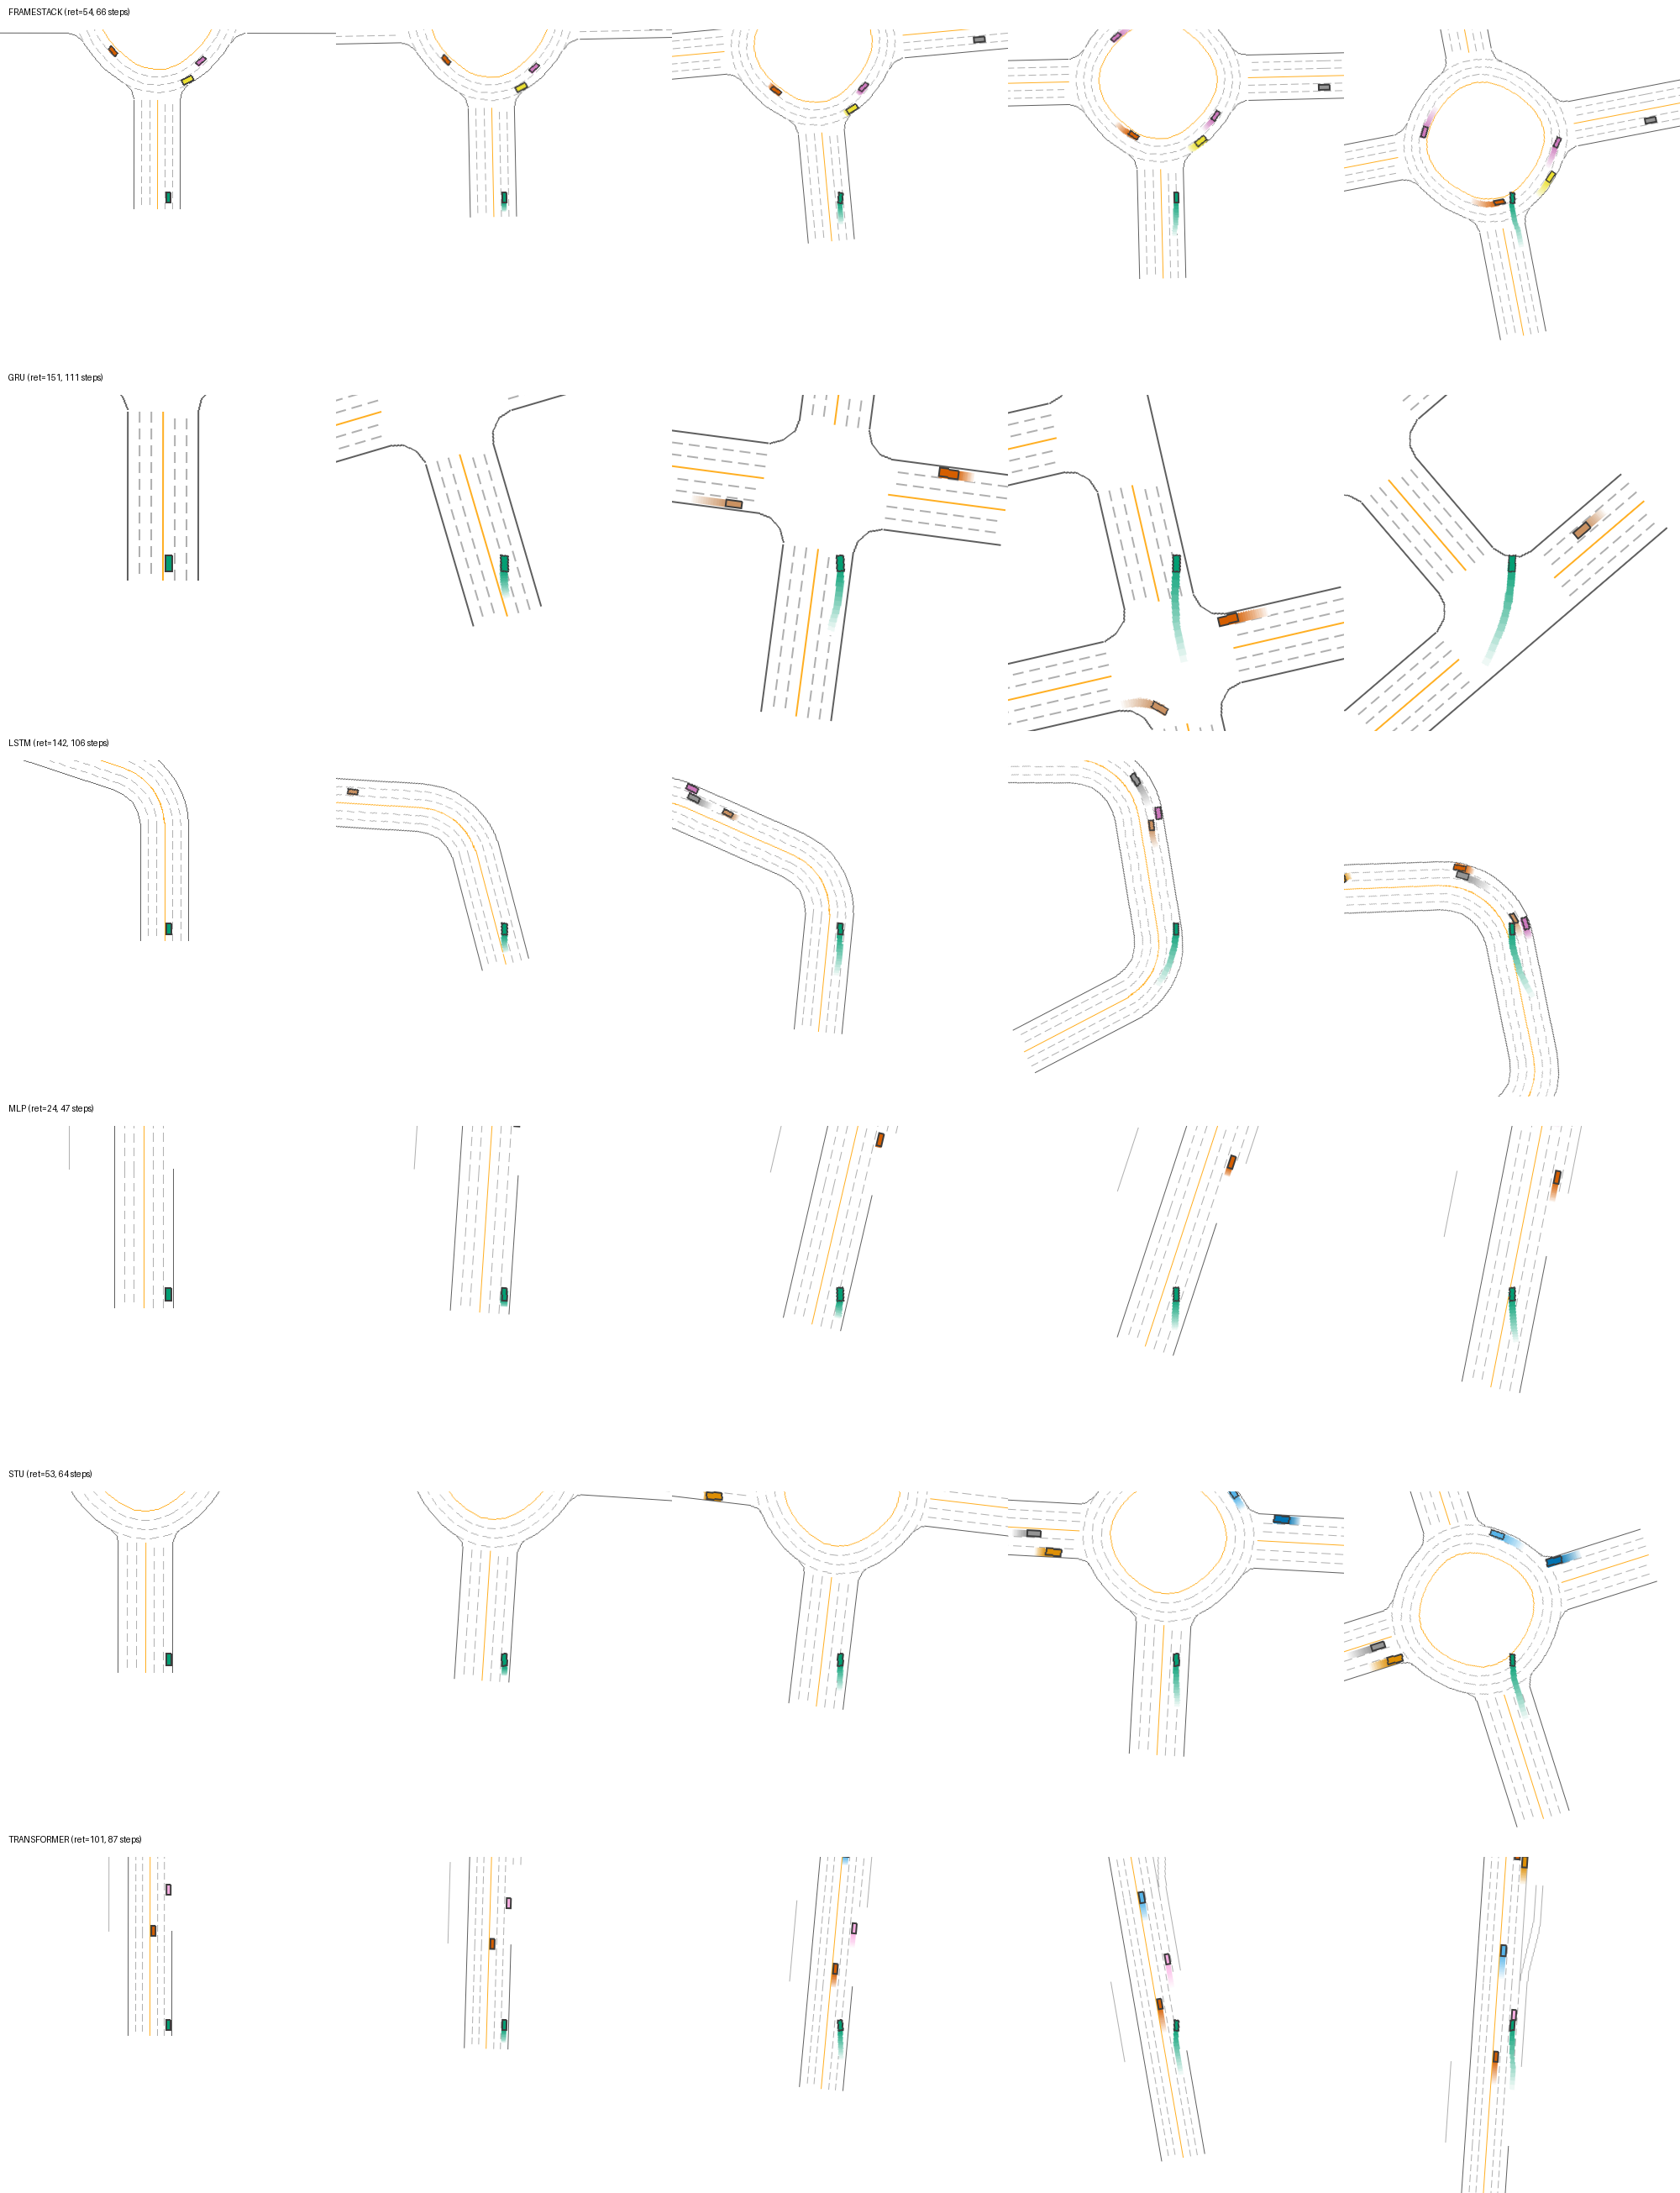
\includegraphics[width=0.7\textwidth]{comparison_metadrive_all.png}
\caption{\textbf{MetaDrive: architecture determines driving competence.} Top-down renderings of a single rollout per architecture (seed 42, 500K teacher). Each row is one architecture; columns show progression through the episode. GRU (row 2, return 151) and LSTM (row 3, return 142) navigate intersections and curves for 100+ steps. MLP (row 5, return 24) drives off-road within 47 steps, confirming that lidar-based driving requires temporal memory. STU (row 4, return 53) crashes at 64 steps despite leading in mean return across all teacher configs (\cref{tab:metadrive})---illustrating that single-rollout visualizations are anecdotal (included for visual intuition only); the table means are the authoritative comparison.}
\label{fig:metadrive-renders}
\end{figure}
\vspace{-6pt}




Video demonstrations of each architecture's locomotion and driving are available at the project repository (\url{https://github.com/wasumayan/wasumind}).


\paragraph{Deployment profiling.}
\label{sec:deployment}

Given our finding that teacher quality matters more than architecture, student selection should be driven by deployment constraints.
For locomotion tasks, GRU is the strongest deployment choice among temporal architectures: fewest parameters (51K), lowest latency (1.26\,ms/step, sufficient for 800\,Hz control loops), and the most robust distillation performance.
Full deployment profiling including latency benchmarks for all architectures is provided in \cref{app:hyperparams}.
